% Sample file on how to use subfiles.
\documentclass[micro_gen.tex]{subfiles}

\begin{document}

\chapter{Microstructure generation}



\begin{figure}
\centering
\begin{subfigure}{.5\textwidth}
  \centering
  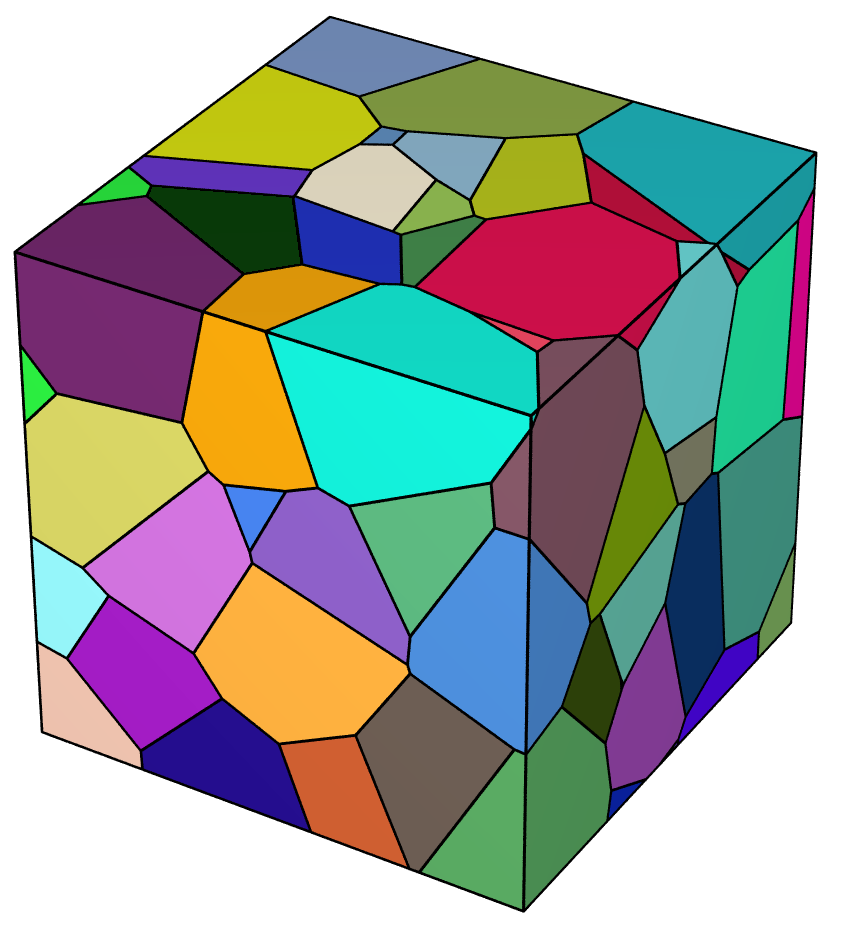
\includegraphics[width=.5\linewidth]{./figures/img_body.png}
  \caption{All polyhedras shown.}
  \label{fig:sub1}
\end{subfigure}%
\begin{subfigure}{.5\textwidth}
  \centering
  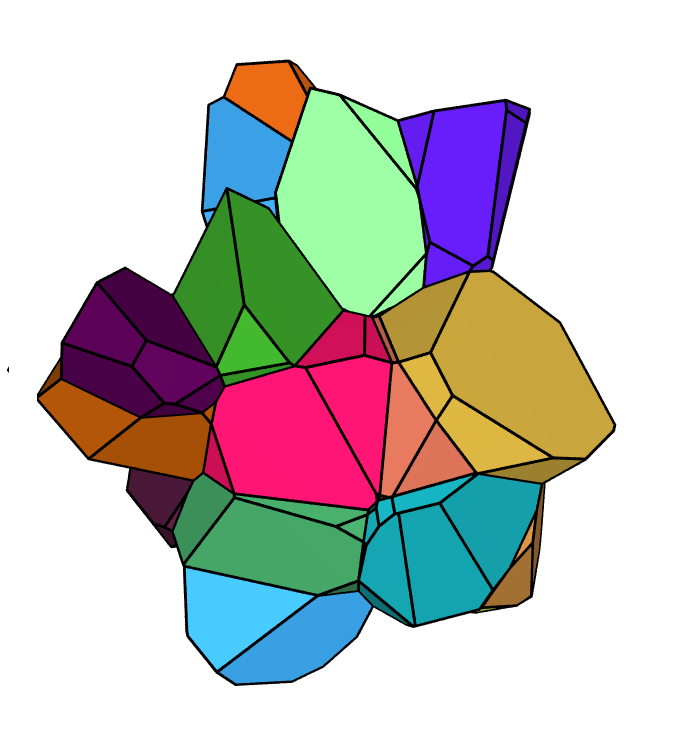
\includegraphics[width=.5\linewidth]{./figures/img_bodyno.png}
  \caption{Polyhedras that are part of the boundary hidden.}
  \label{fig:sub2}
\end{subfigure}
\caption{Voronoi tesselation with 500 generation points bounded by a cube}
\label{fig:test}
\end{figure}

The open source software Neper \cite{neper} was used to both generate the microstructure and mesh it. In Neper it is possible to explicitly give the seeds of the voronoi tesselation as well as generate random seeds. The microstructure can then be meshed which is done in a way to maximize the quality of the mesh. A more detailed description of the meshing process can be read in the referenced paper. There is some freedom in how the mesh is generated. The mesh courseness can be controlled as well as some regularization parameters which determine the worst quality allowed of the elements. The mesh generated is made up of tetrahedrons of first or second order. In the generated mesh file there are also element and node sets available to us. What can be read is the what grain each element is part of, the nodes on the six boundaries of the bounding cube and the nodes that are in the faces between two grains.

\end{document}
